\subsection{List of experiments}
\begin{frame}{List of experiments}
	\begin{enumerate}
		\item<alert@2> Rock-paper-scissors model in bacterial community
		\item Evolutionary games theory: Hawk and Dove example
		\item The Lotka-Volterra model of competition between two competing species
		\item Game Theory with social dilemmas of tumour acidity and vasculature
		\item Prostate cancer tumour–stroma interactions
		\item<alert@2> Evolutionary Dynamics of Tumor-Stroma Interactions in Multiple Myeloma
	\end{enumerate}
\end{frame}

\subsection{An experiment with bacteria}

\begin{frame}{Rock-paper-scissors game in bacterial community}

    \begin{itemize}
        \item \textbf{Title:} Local dispersal promotes biodiversity in a real-life game of rock–paper–scissors.
        \item \textbf{Authors:} Benjamin Kerr, Margaret A. Riley, Marcus W. Feldman, Brendan J. M. Bohannan.
        \item Three competing species of bacterias with relationships similar to rock-paper-scissors game.
    \end{itemize}
            \begin{figure}[t]
    			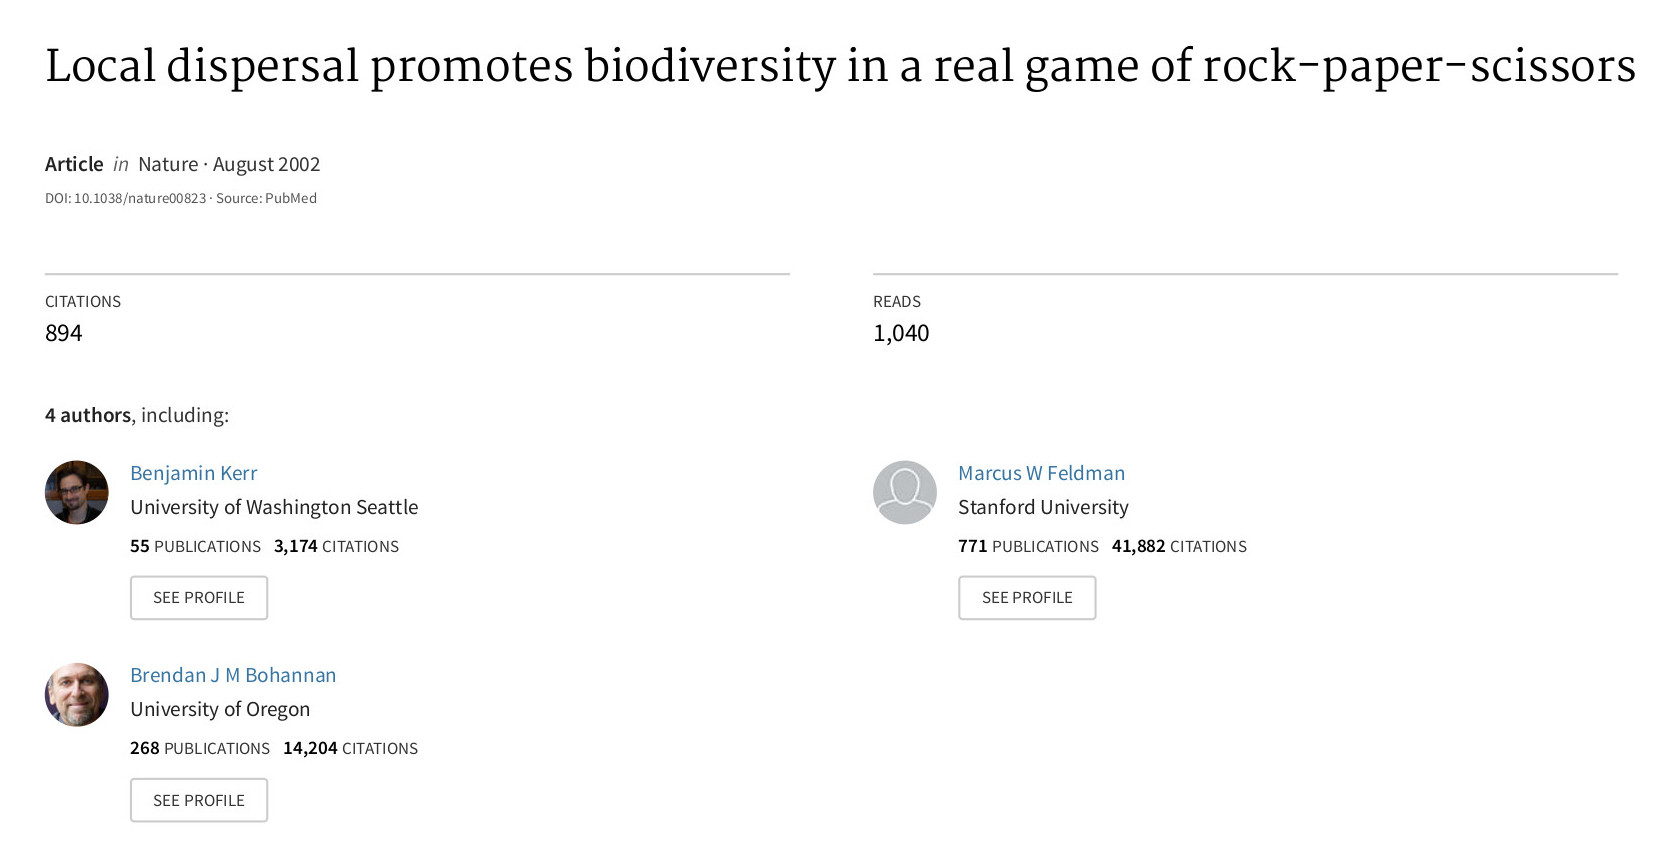
\includegraphics[scale=0.7]{img/paper_bacteria.jpg}
    		\end{figure}
\end{frame}

\begin{frame}{Rock-paper-scissors game in bacterial community}
    \begin{itemize}
		\item Three types of populations of \textit{E. coli}: 
		\begin{itemize}
			\item Wild-type bacterias (WT): colicin-sensitive bacterias, hence, they are killed by colicin. 
			\item Colicinogenic bacterias (C): produce colicin toxin, a colicin-specific inmunity protein and a lysis protein which causes partial cell lysis and the release of the colicin.
			\item Colicin-resistant bacterias (R): WT bacterias who have mutated getting membrane translocators of colicin.
		\end{itemize}
		\item Parameters that describe the relationships of WT-C-R community:
		\begin{itemize}
			\item $a$: advantage of WT over R $\Rightarrow$ R have costs in their fitness because the resistance consumes a lot of energy and WT have not this problem.
			\item $b$: advantage of C over WT $\Rightarrow$ C are able to kill WT.
			\item $c$: advantage of R over C $\Rightarrow$ R are resistant to colicin produced by C. 
		\end{itemize}
		
    \end{itemize}
\end{frame}

\begin{frame}{Rock-paper-scissors game in bacterial community}
	\begin{columns}
		\begin{column}{0.5\textwidth}
			\begin{center}
				In summary, we have the relationships of rock-paper-scissors game:
			\end{center}
			\begin{figure}
				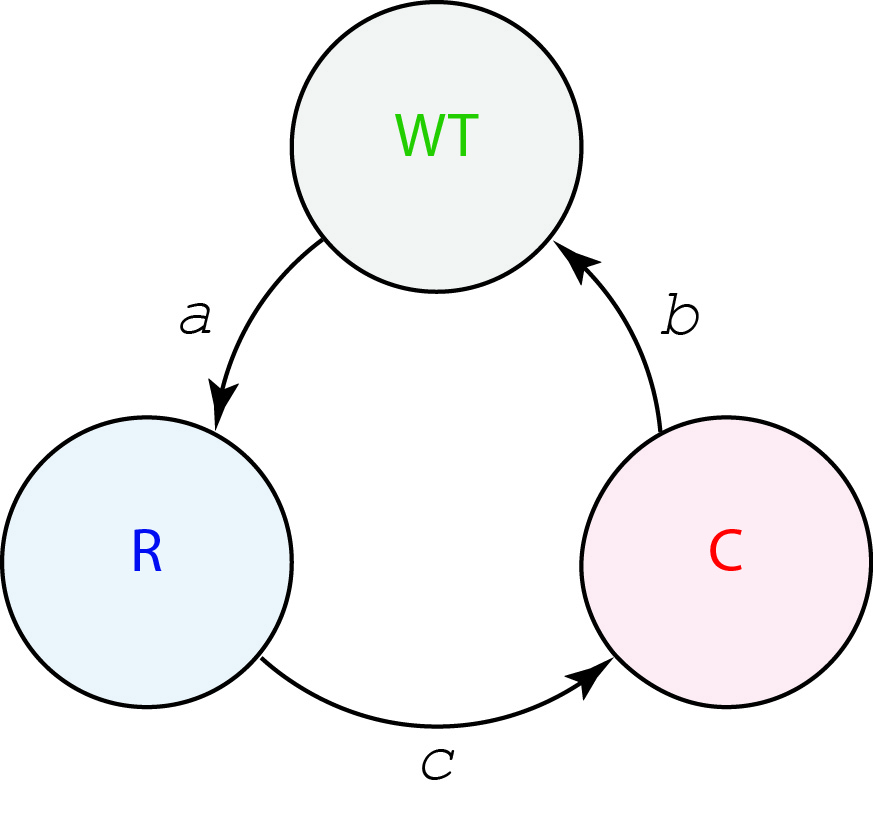
\includegraphics[scale=0.12]{img/figure_rock-scissor-paper.jpg}			
			\end{figure}
		\end{column}
		\begin{column}{0.5\textwidth}
			\begin{center}
				And the resulting equations:
			\begin{align*}
				W\left(WT\right) = 1 + af_3 - bf_2\\
				W\left(C\right) = 1 + bf_1 - cf_3\\
				W\left(R\right) = 1 + cf_2 - af_1\\
			\end{align*}
			where $f_1$, $f_2$ and $f_3$ are the frequencies of WT, C and R, respectively. 
			\end{center}
		\end{column}
	\end{columns}
	\pause
	\begin{center}
		{\LARGE $\Downarrow$\\}
		%% Meter alert %%
		\begin{block}
			{\centering
				\textit{allFitnessEffect} and \textit{oncoSimulIndiv} functions
			}
		\end{block}
	\end{center}	
\end{frame}

\subsection{An experiment with cells}

\begin{frame}{Tumor-Stroma Interactions}

    \begin{itemize}
        \item \textbf{Title:} Evolutionary Dynamics of Tumor-Stroma Interactions in Multiple Myeloma.
        \item \textbf{Authors:} Javad Salimi Sartakhti, Mohammad Hossein Manshaei, Soroosh Bateni, Marco Archetti.
        \item Cancer cells and stromal cells cooperate by exchanging diffusible factors.
        \begin{itemize}
            \item Frequency-dependent selection that can be studied in the framework of evolutionary game theory.
        \end{itemize}
    \end{itemize}
    
\end{frame}

\begin{frame}{Tumour-Stroma Interactions: payoff functions}
    \begin{itemize}
        \item There are $n$ phenotypes in a population denoted by $\{ P_1, \ldots, P_n \}$.
        \item Each phenotype can produce one diffusible factor $\{ G_1, \ldots, G_n \}$.
        \item Each diffusible factor $j$ has a different effect $r_{i,j}$ on the other phenotypes $i$.
        \item The cost for $P_i$ for growth factor $G_i$ is denoted as $c_i$.
        \item $M$ is the number of cells within the diffusion range.
        \begin{itemize}
            \item There are $M_j$ individuals of type $P_j$ among the other group members.
        \end{itemize}
        \item The payoff for strategy $P_j$ is:
        \begin{align*}
            \pi_{P_j}(M_1,\ldots,M_n)=\frac{(M_j+1)\times c_j}{M}r_{j,j} + \sum_{i=1, i \neq j}^n \frac{M_i \times c_i}{M}r_{j,i} - c_j \;.
        \end{align*}
    \end{itemize}
\end{frame}

\begin{frame}{Tumour-Stroma Interactions: dynamics}
    \begin{columns}
        \begin{column}{0.4\textwidth}
             \begin{itemize}
                \item Malignant plasma cells.
                \item Osteoblasts.
                \item Osteoclasts.
                \item Growth factors:
                \begin{itemize}
                    \item Autocrine effects.
                    \item Paracrine effects. 
                \end{itemize}
            \end{itemize}
        \end{column}
        \begin{column}{0.6 \textwidth}
            \begin{figure}[t]
                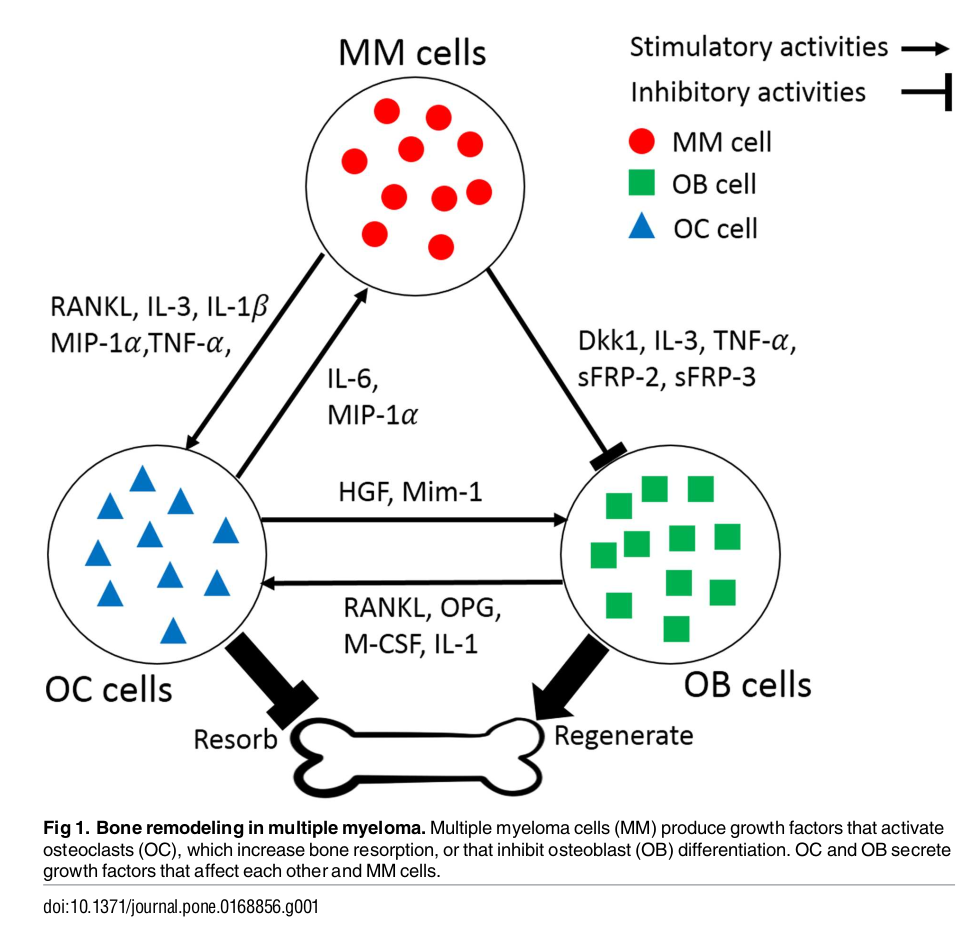
\includegraphics[width=0.9\linewidth]{img/tumour_stroma_interactions.png}
            \end{figure}
        \end{column}
    \end{columns}
\end{frame}



\begin{frame}{Tumour-Stroma Interactions: Scenario 1}
    \begin{itemize}
        \item $c_1<c_2<c_3$ (a common occurrence in multiple myeloma).
        \item In the presence of a small number of MM cells, the stable point on the OB-OC border becomes a saddle point and clonal selection leads to a stable coexistence of OC and MM cells.
    \end{itemize}
    
    \begin{columns}
        \begin{column}{0.4\textwidth}
            \begin{figure}[t]
                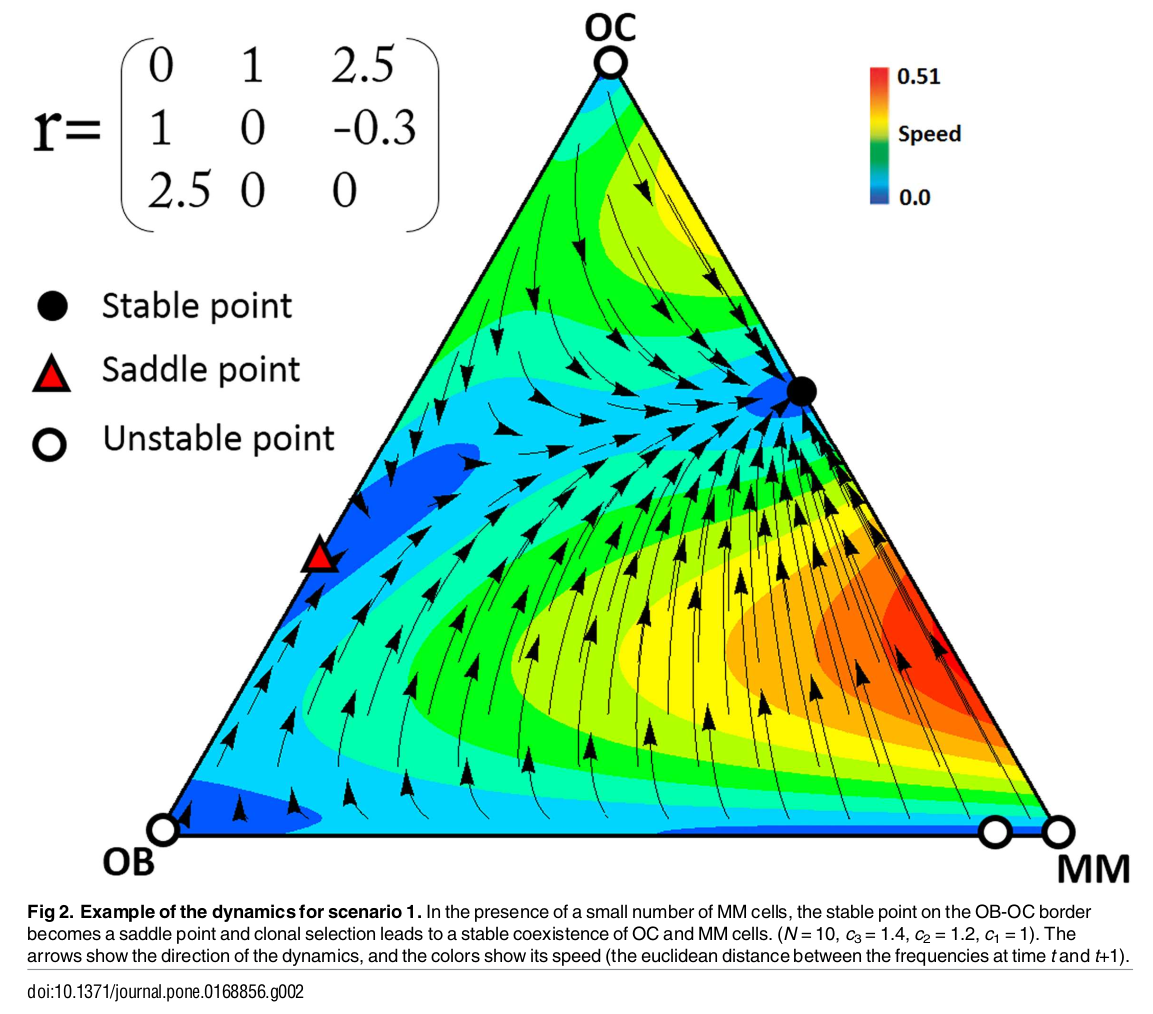
\includegraphics[width=0.9\linewidth]{img/Scenario1.png}
            \end{figure}
        \end{column}
        \begin{column}{0.6\textwidth}
            \begin{figure}[t]
                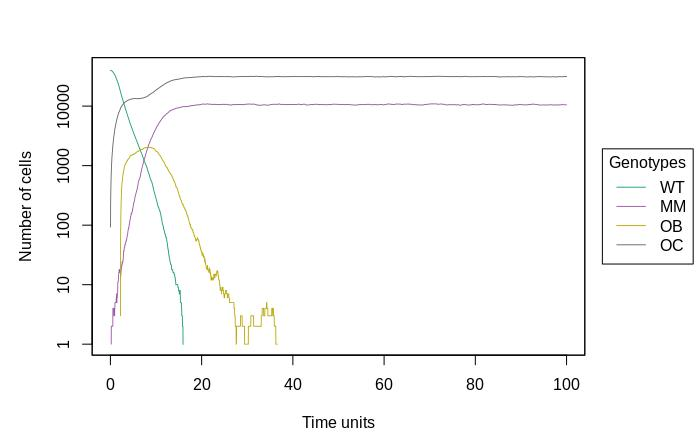
\includegraphics[width=0.9\linewidth]{img/scenario1_tr.jpg}
            \end{figure}
        \end{column}
    \end{columns}
\end{frame}

\begin{frame}{Tumour-Stroma Interactions: Scenario 2}
    \begin{itemize}
        \item $c_1=c_2=c_3$.
        \item The game has one polymorphic stable point between OB and OC. In this case, clonal selection leads to the regular OC-OB balance and prevents invasion of MM cells.
    \end{itemize}
    
    \begin{columns}
        \begin{column}{0.4\textwidth}
            \begin{figure}[t]
                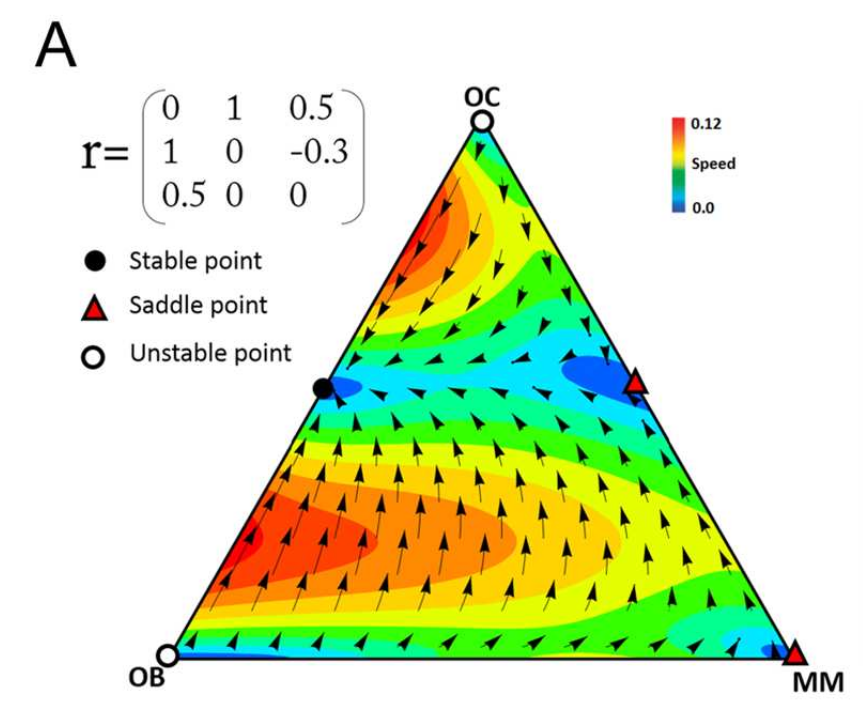
\includegraphics[width=0.9\linewidth]{img/Scenario2.png}
            \end{figure}
        \end{column}
        \begin{column}{0.6\textwidth}
            \begin{figure}[t]
                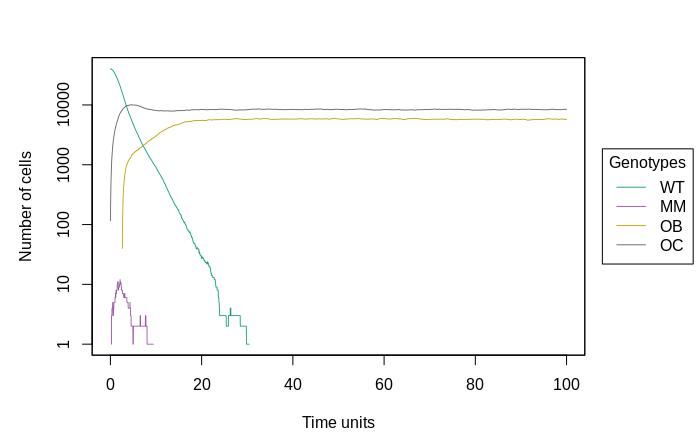
\includegraphics[width=0.9\linewidth]{img/scenario2_tr.jpg}
            \end{figure}
        \end{column}
    \end{columns}
\end{frame}